\FloatBarrier
\subsection{Kurvenauswertung}



%T_high I_low U_längs
%B1 = 1.83143 +- 0.00449283
%U1 = 0.02058
%B2 = 3.29231 +- 0.00382163
%U2 = 0.04827
\begin{figure}
\label{}
\centering
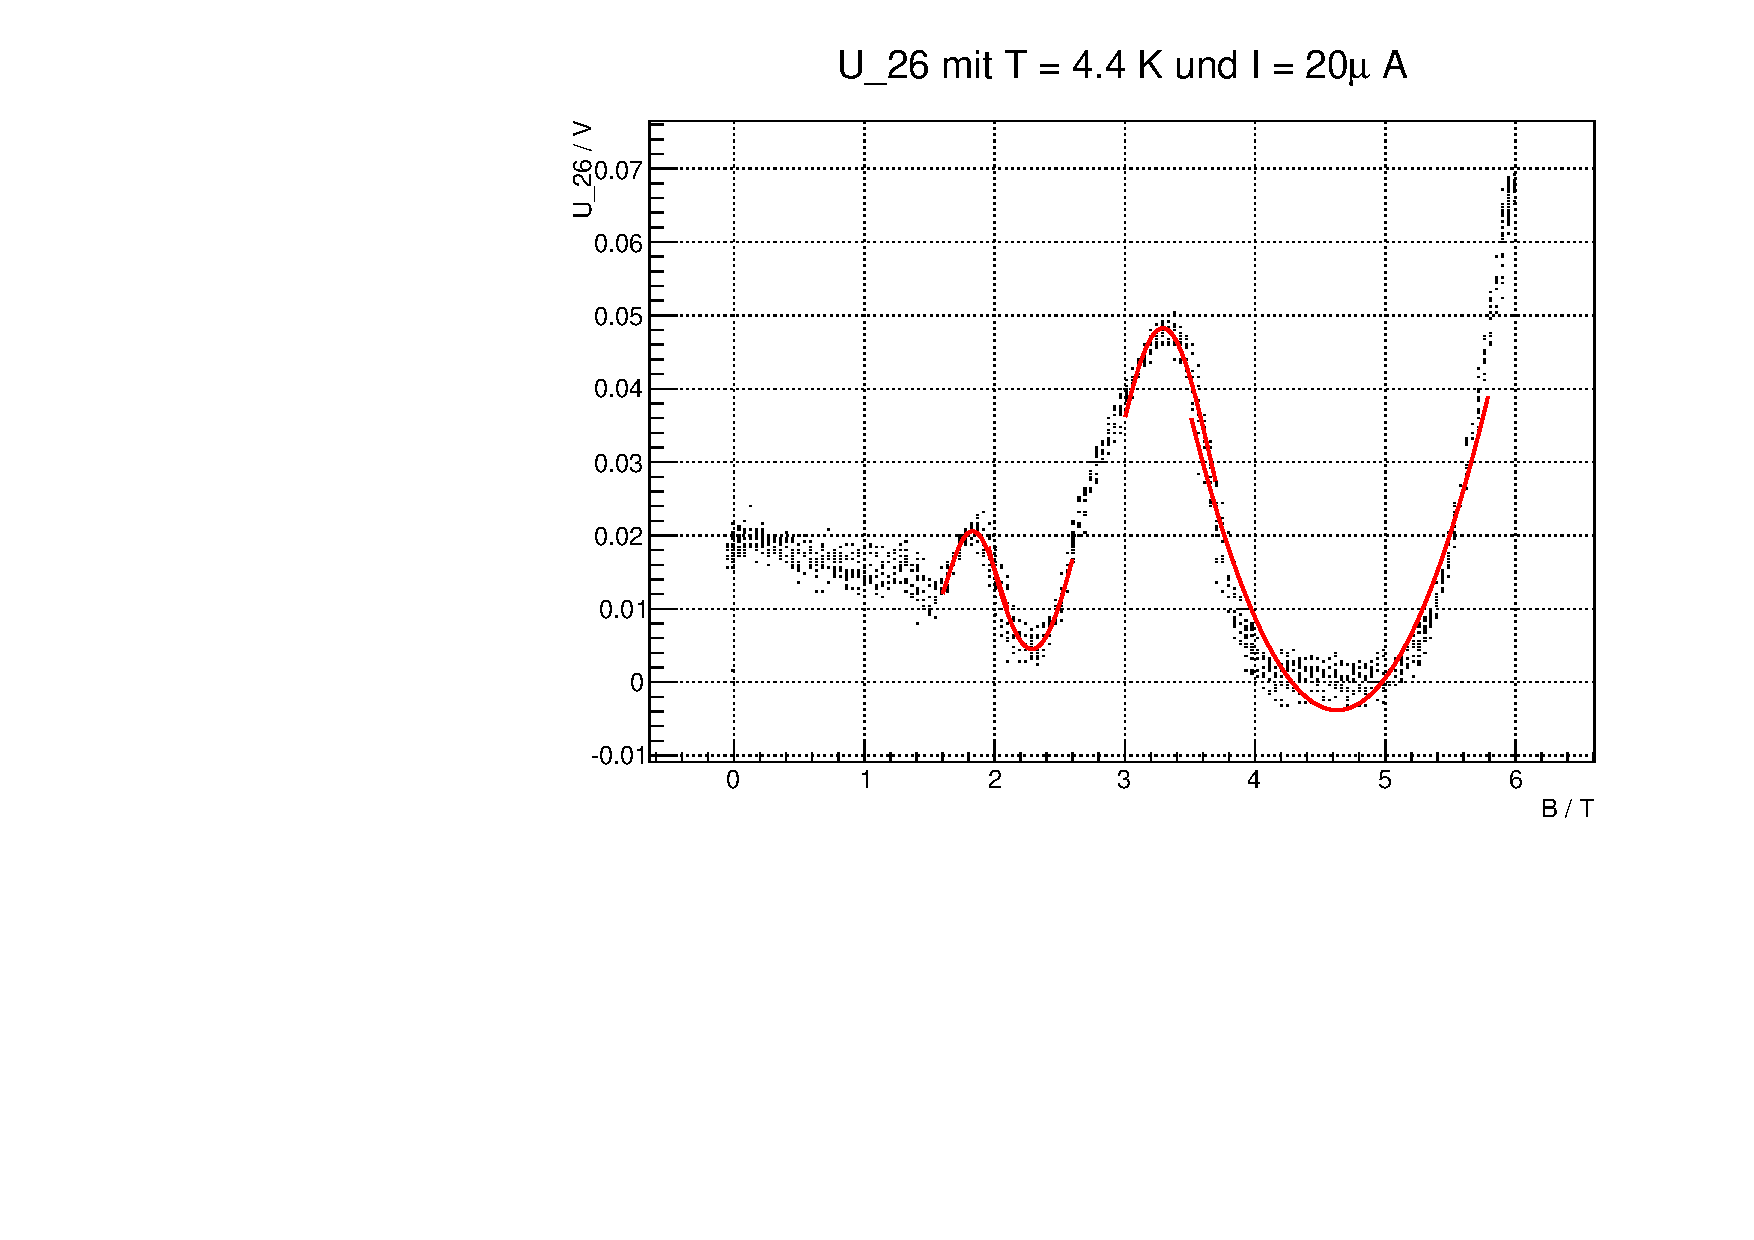
\includegraphics[scale = 0.5]{../plots/U_26_20muA_4400mK.pdf}
\caption{$\text{V}_x$ für I=20 $\mu$A und T=4.4 K}
\end{figure}

%T_high I_high U_längs
%B1 = 1.85495 +- 0.00420536
%U1 = 0.09374
%B2 = 3.45507 +- 0.00343915
%U2 = 0.19468
\begin{figure}
\label{}
\centering
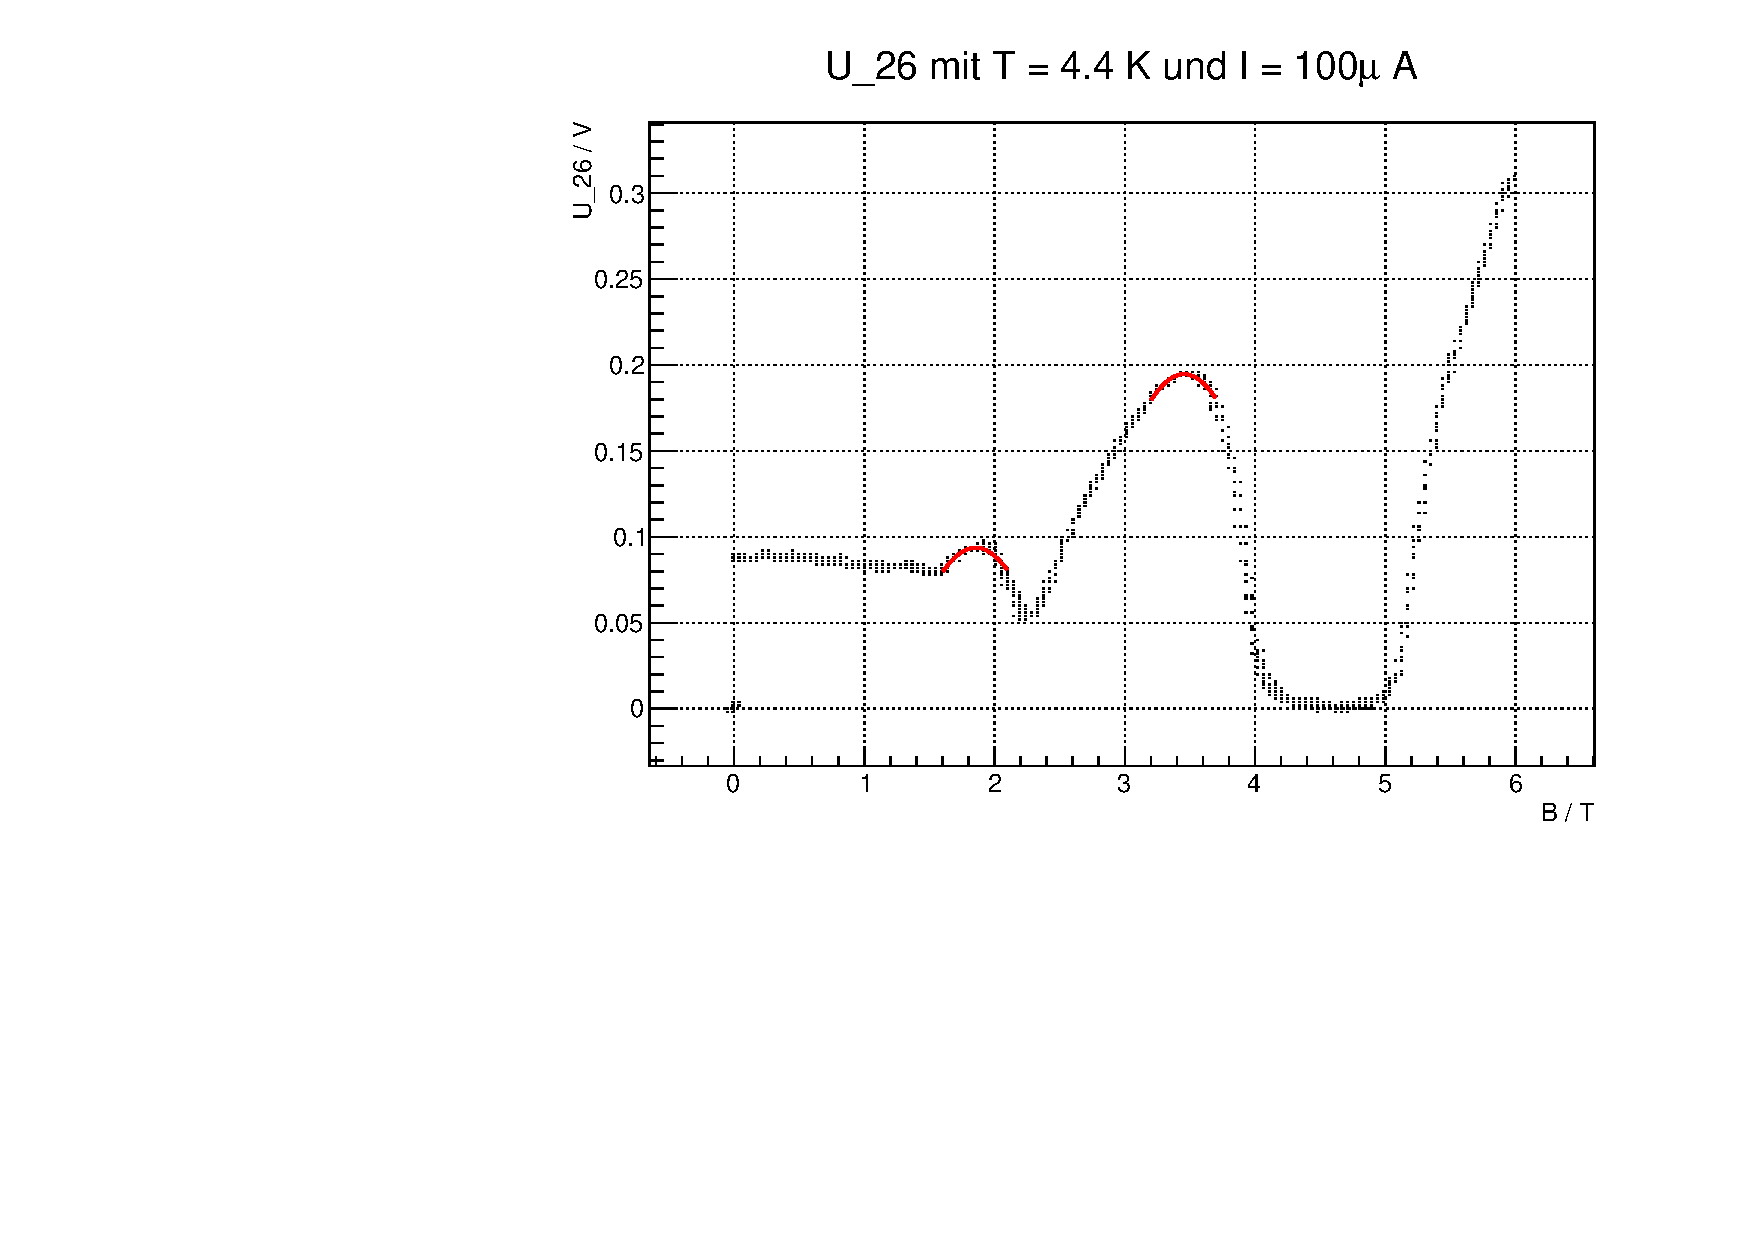
\includegraphics[scale = 0.5]{../plots/U_26_100muA_4400mK.pdf}
\caption{$\text{V}_x$ für I=100 $\mu$A und T=4.4 K}
\end{figure}

%missing
%%T_low I_low U_längs
%\begin{figure}
%\label{}
%\centering
%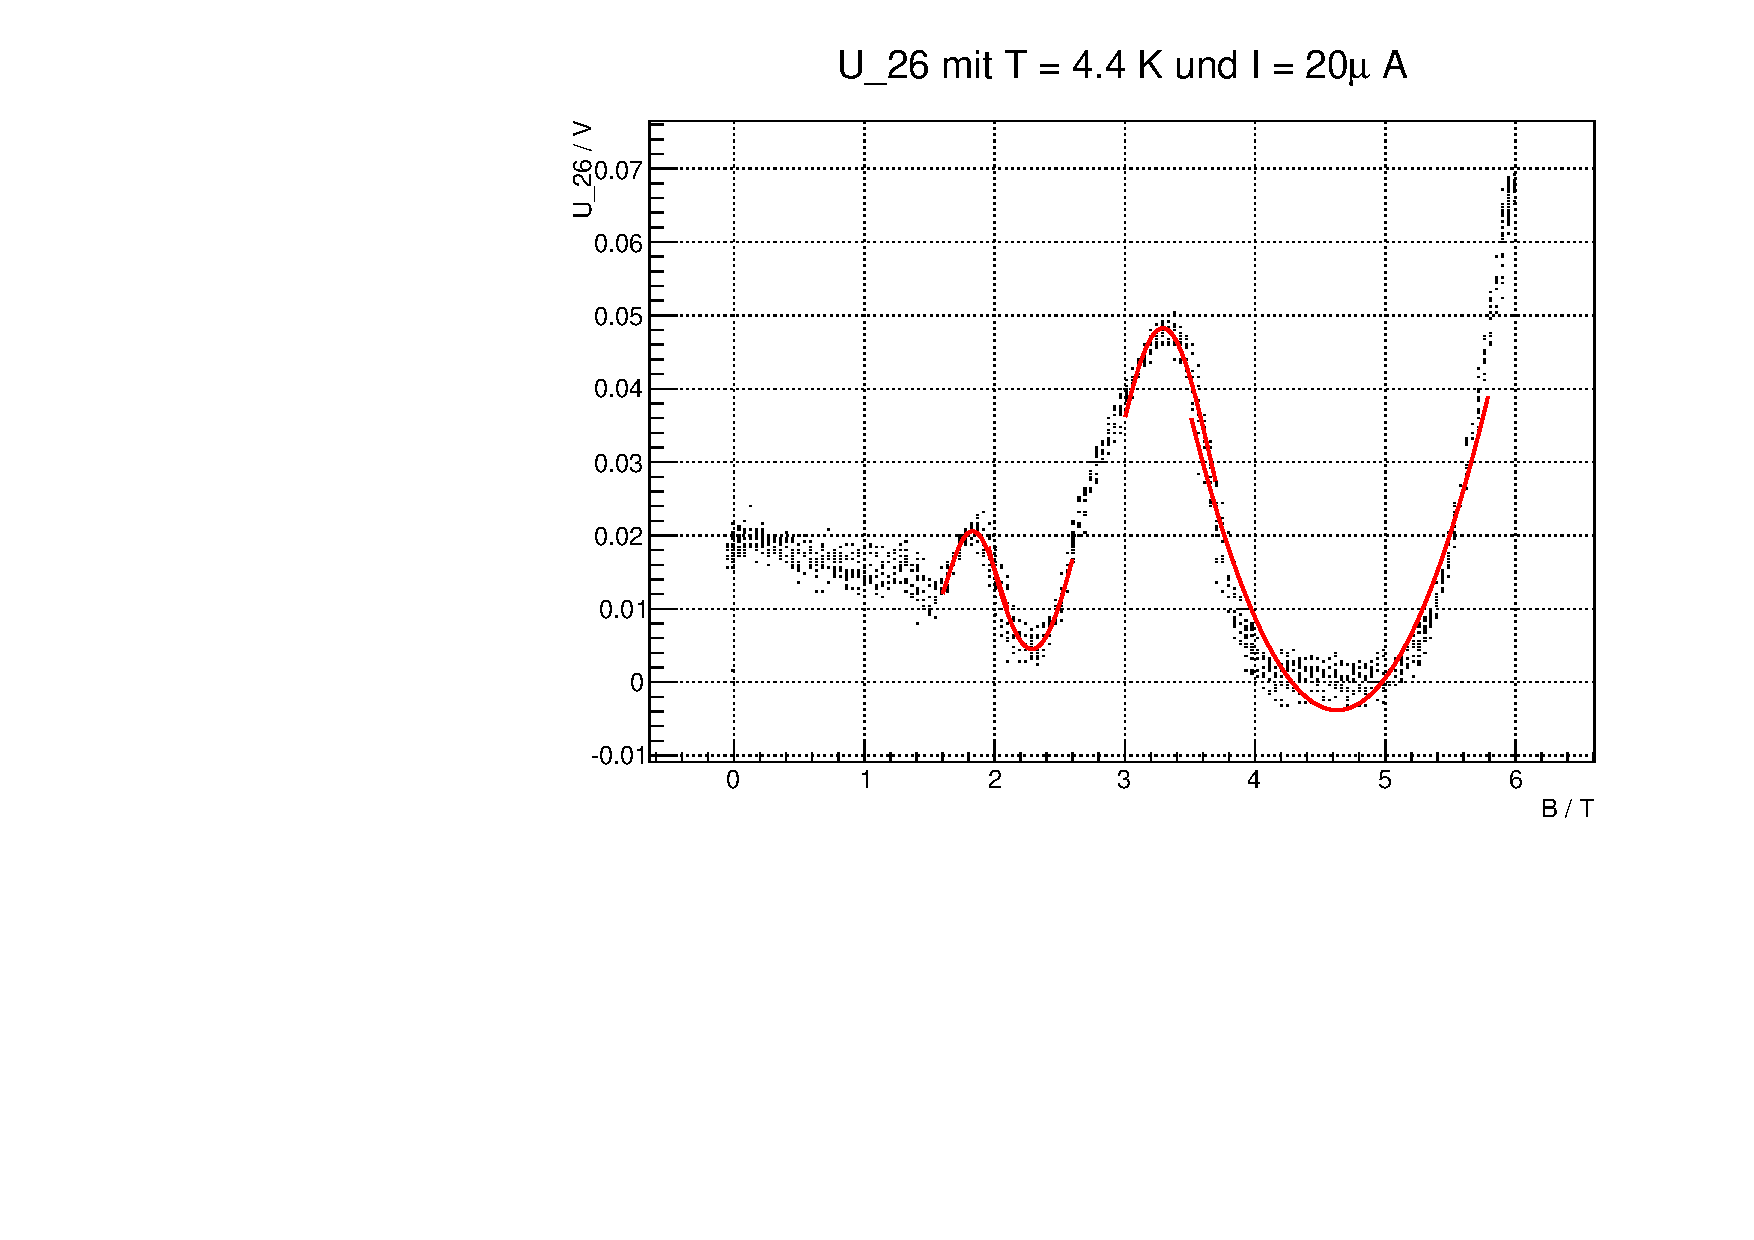
\includegraphics[scale = 0.5]{../plots/U_26_20muA_4400mK.pdf}
%\caption{}
%\end{figure}

%T_low I_high U_längs
%B1 = 2.36875 +- 0.00691555
%U1 = 0.095265
%B2 = 4.40606 +- 0.00615656
%U2 = 0.202313
\begin{figure}
\label{}
\centering
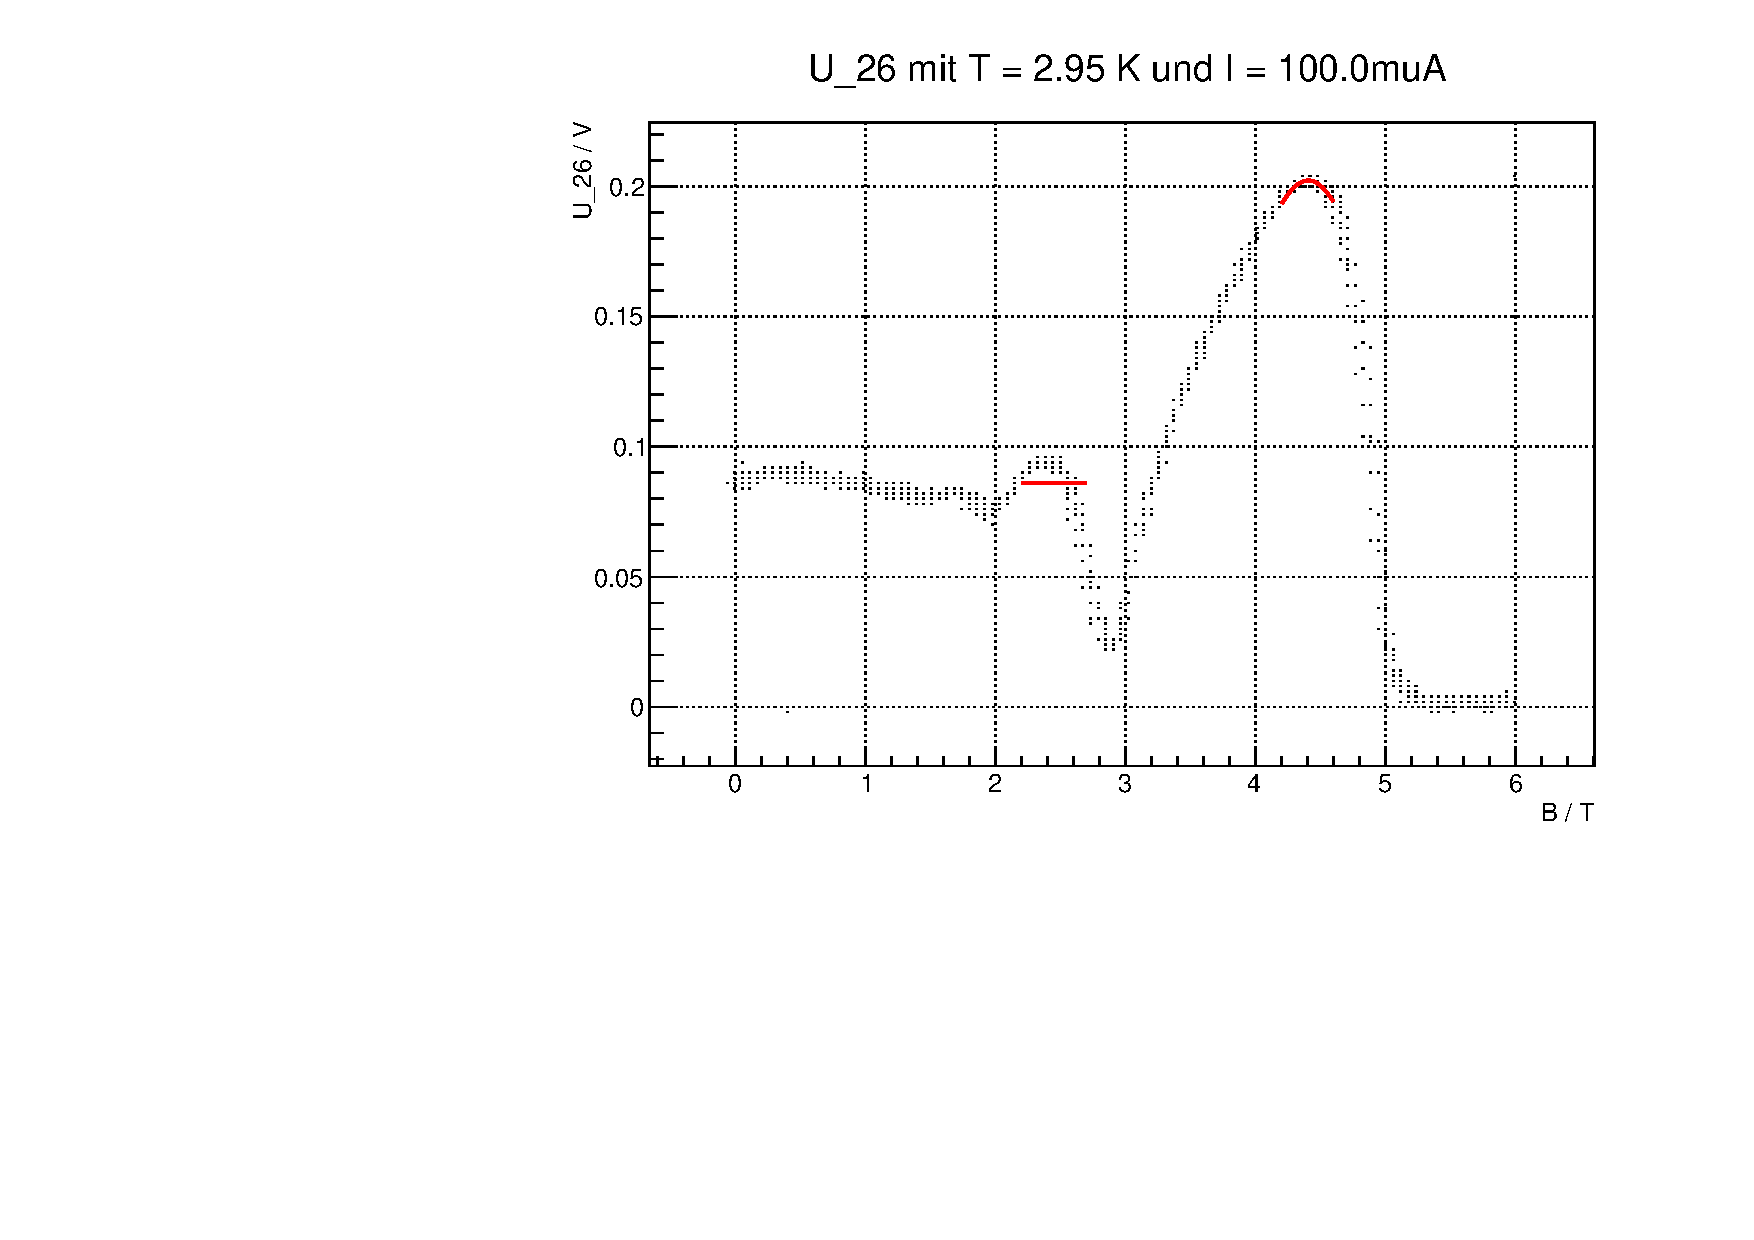
\includegraphics[scale = 0.5]{../plots/U_26_100muA_2950mK.pdf}
\caption{$\text{V}_x$ für I=100 $\mu$A und T=2.95 K}
\end{figure}


%T_high I_low U_hall
%U1 = 0.131545 +- 0.000282565
%U2 = 0.263575 +- 0.000178472
\begin{figure}
\label{}
\centering
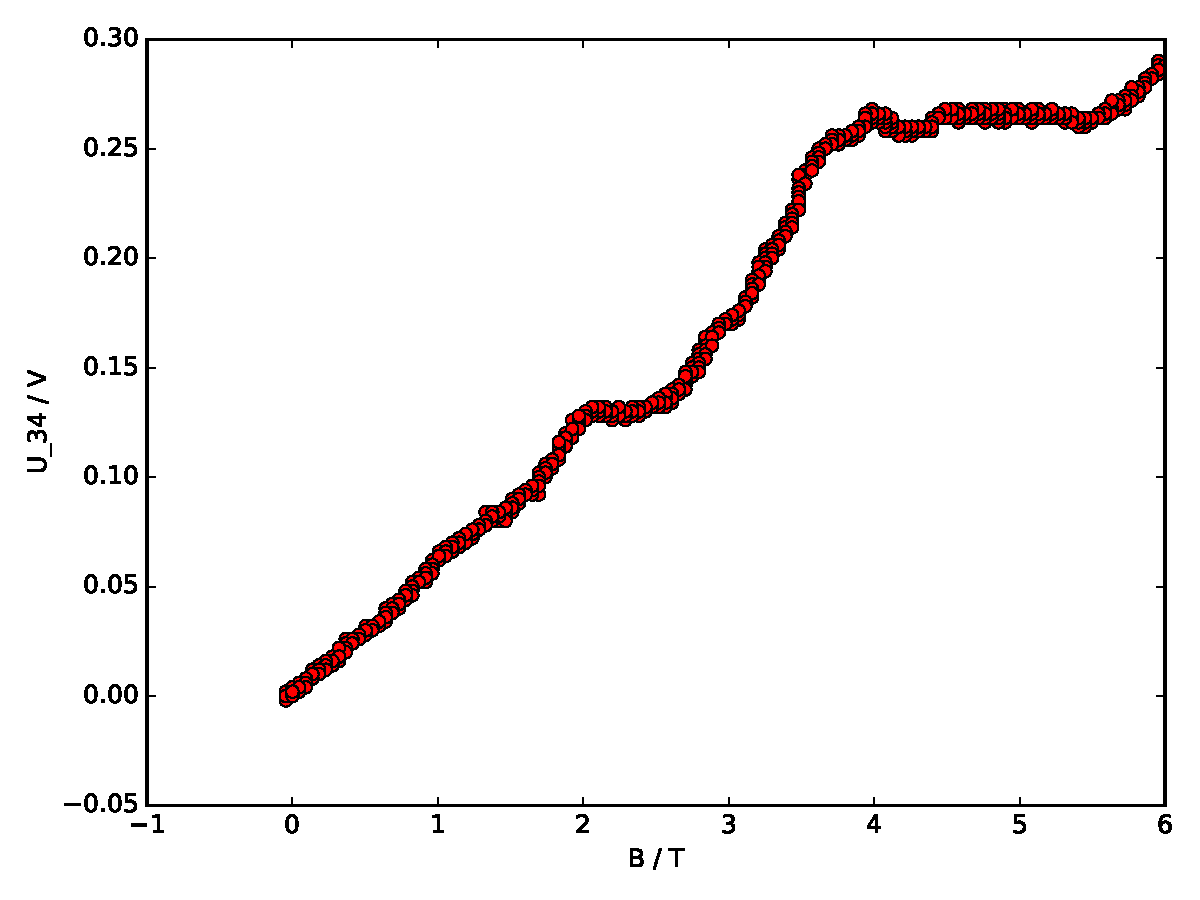
\includegraphics[scale = 0.5]{../plots/U_34_20muA_4100mK.pdf}
\caption{$\text{V}_H$ für I=20 $\mu$A und T=4.1 K}
\end{figure}

%T_high I_high U_hall
%U1 = 0.656545 +- 0.00117472
%U2 = 1.30261 +- 0.000290939
\begin{figure}
\label{}
\centering
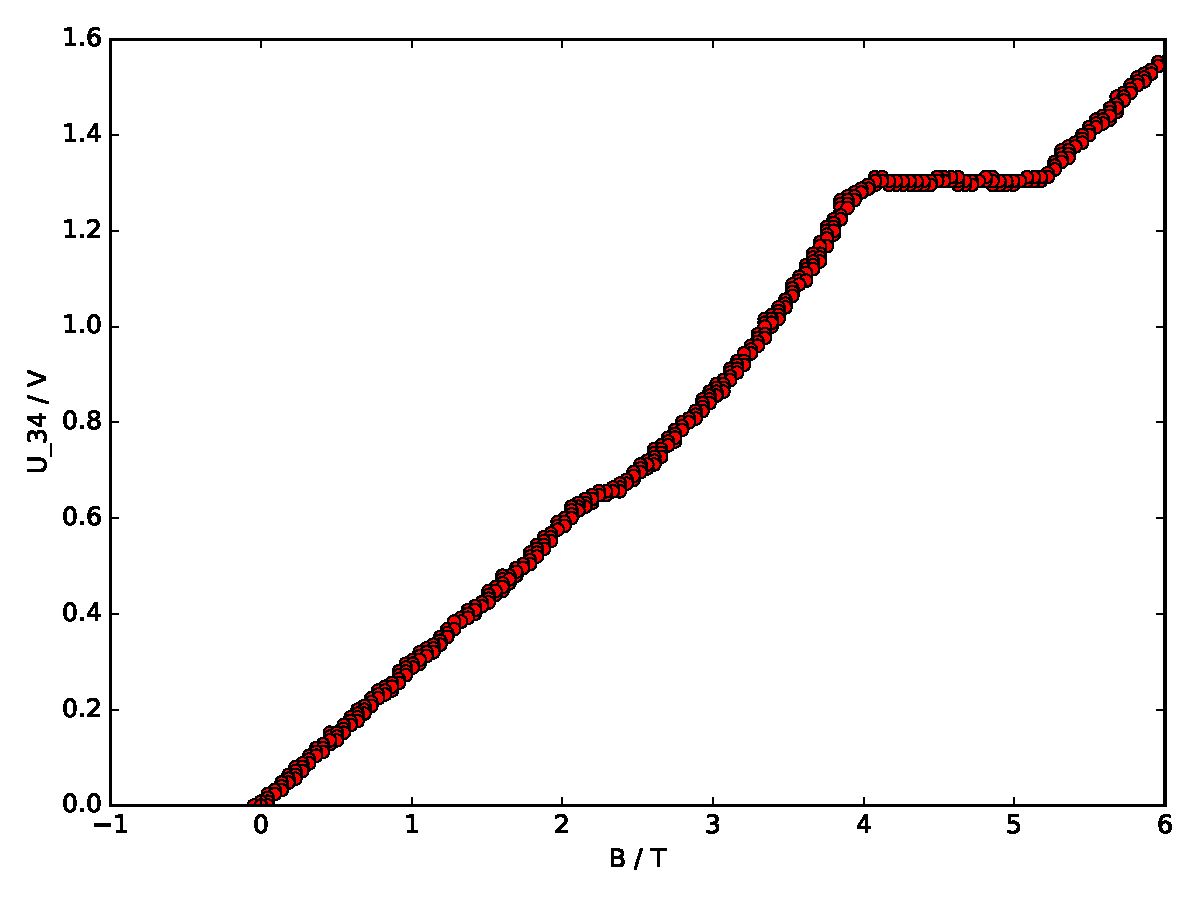
\includegraphics[scale = 0.5]{../plots/U_34_100muA_4400mK.pdf}
\caption{$\text{V}_H$ für I=100 $\mu$A und T=4.4 K}
\end{figure}

%T_low I_low U_hall
%U1 = 0.0841778 +- 0.000260708
%U2 = 0.136876 +- 0.000196899
%U3 = 0.25837 +- 8.46565e-05
\begin{figure}
\label{}
\centering
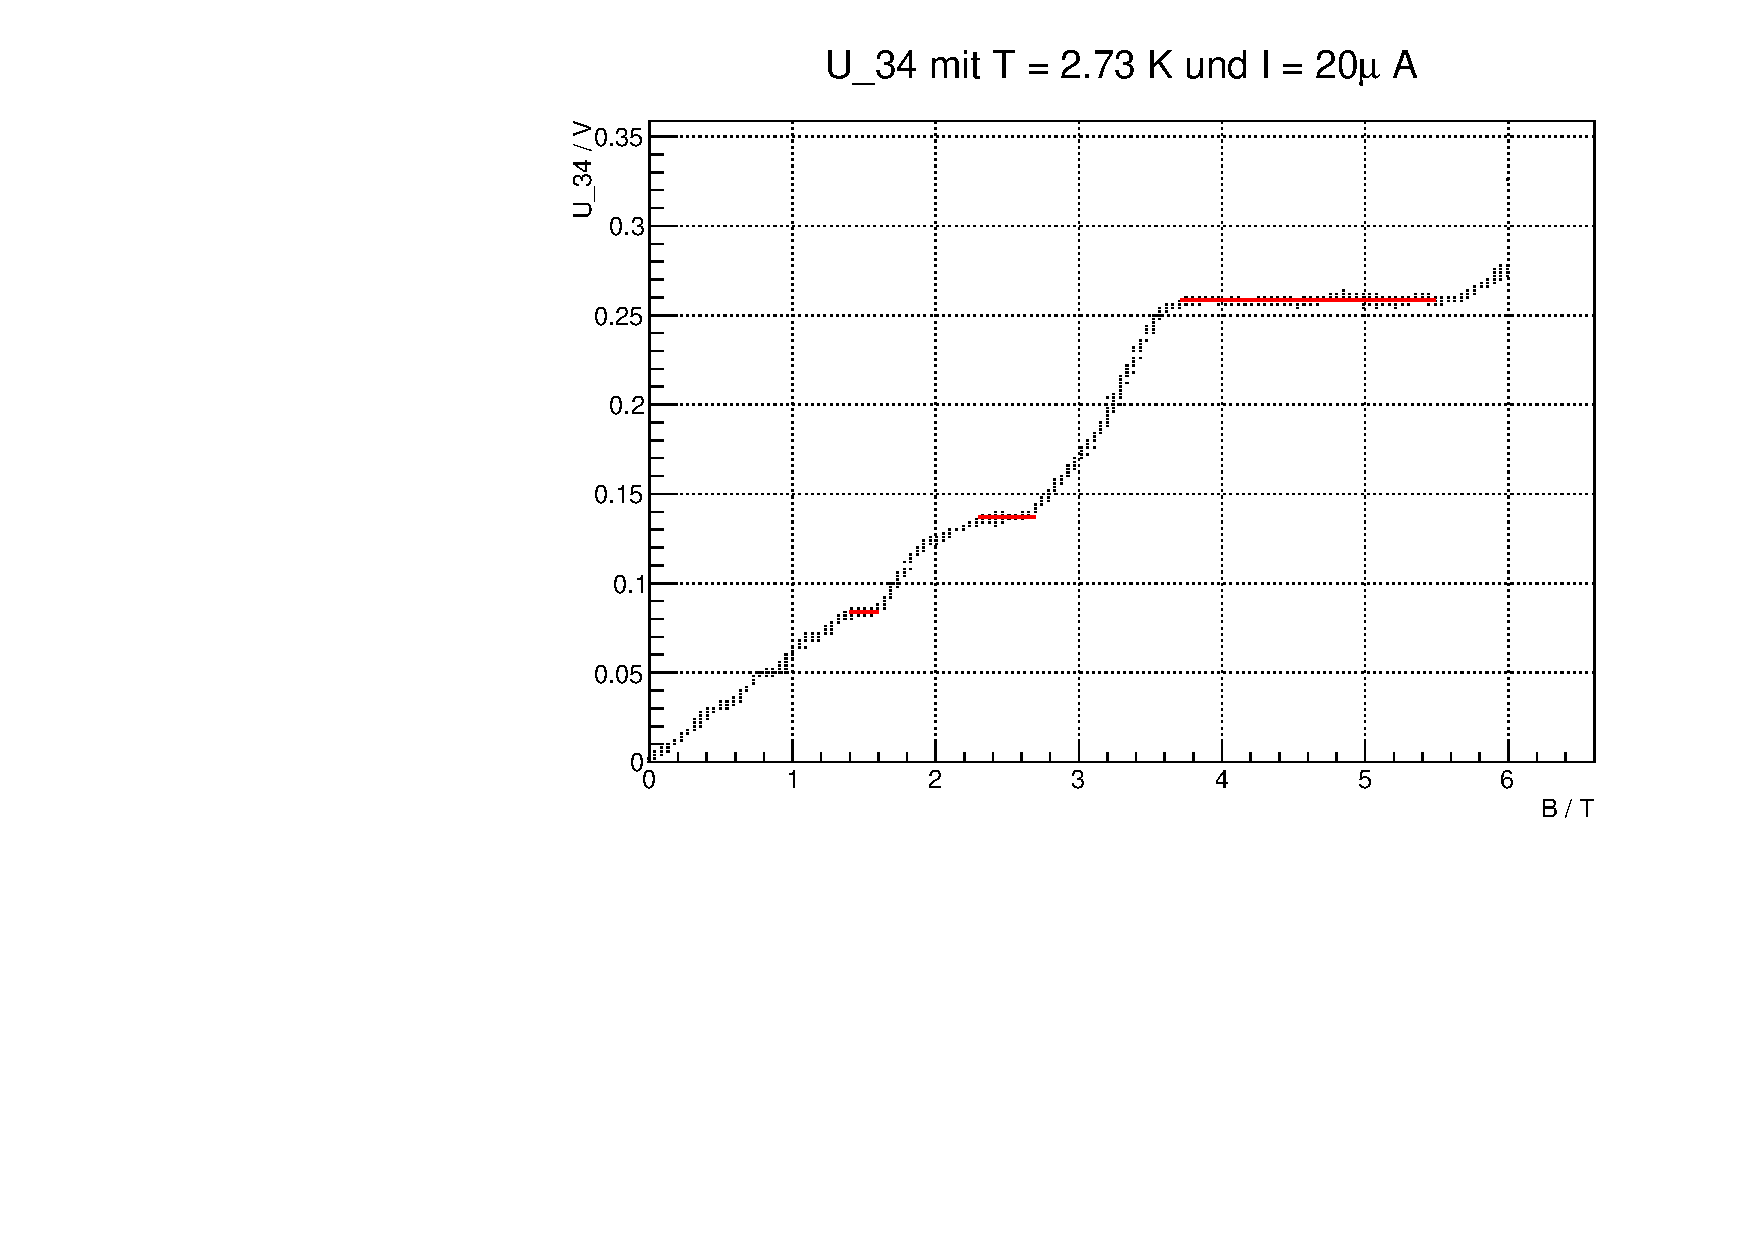
\includegraphics[scale = 0.5]{../plots/U_34_20muA_2730mK.pdf}
\caption{$\text{V}_H$ für I=20 $\mu$A und T=2.73 K}
\end{figure}

%T_low I_high U_hall
%U1 = 0.645867 +- 0.00088919
%U2 = 1.30603 +- 0.00025627
\begin{figure}
\label{}
\centering
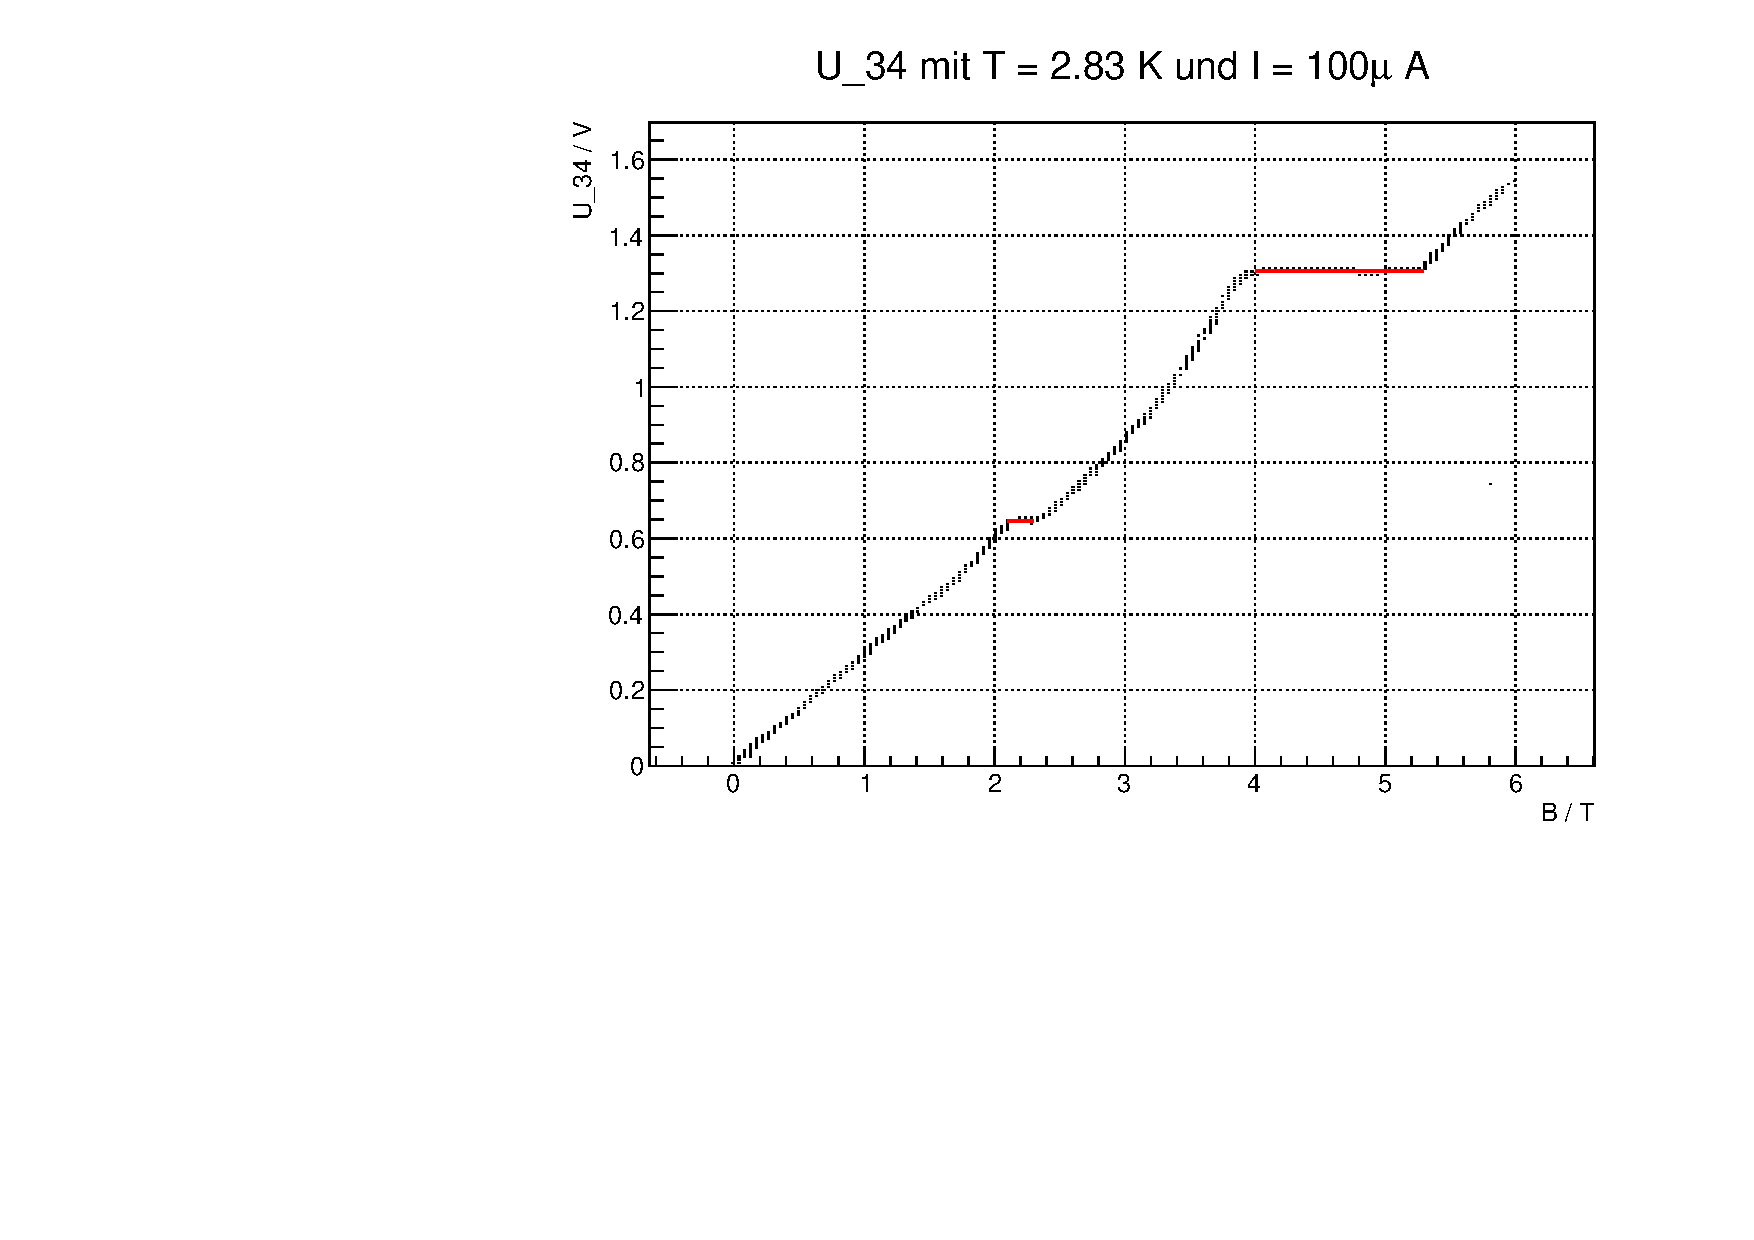
\includegraphics[scale = 0.5]{../plots/U_34_100muA_2830mK.pdf}
\caption{$\text{V}_H$ für I = 100 $\mu$A und T=2.83 K}
\end{figure}


\FloatBarrier


\subsubsection{Längsspannung}

\subsubsection{Hall-Plateaus}

\subsubsection{Ladungsträgerkonzentration}

\subsection{Feinstrukturkonstante}

\subsection{Literaturvergleich}
